\documentclass[10pt]{article}

\usepackage{amsmath}
\usepackage{fullpage}
\usepackage{array}
\usepackage{graphicx}
\usepackage{gensymb}
\usepackage{booktabs}
\usepackage{gensymb}
\usepackage{graphicx}

\graphicspath{ {../Images/} }

\date{2014-6-22}
\pagestyle{empty}
\setlength{\parindent}{0pt}

\begin{document}
\begin{center}
\begin{Large}\textbf{Physical Science 303 - Makeup Assignment}\end{Large} \\
\smallskip
%\begin{large} Acceleration \end{large}
\end{center}
%%%%%%%
Draw the free body diagrams (FBD) corresponding to the following physical systems.  Assume the gravitational force.  All surfaces are frictionless.
 \begin{enumerate}
\item Mass kept on the floor
\begin{figure}[h]
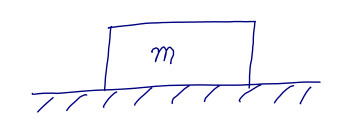
\includegraphics[scale=.5]{fbdmass}
\centering
\end{figure}

\item Two masses supported by the walls
\begin{figure}[h]
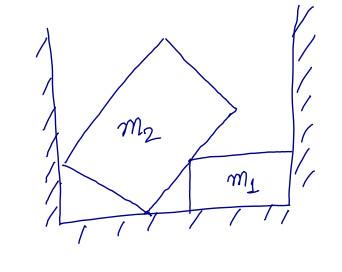
\includegraphics[scale=.5]{fbdmass2}
\centering
\end{figure}

\item Masses hung from the pulley.  Draw the FBD for both the masses and the pulley
\begin{figure}[h]
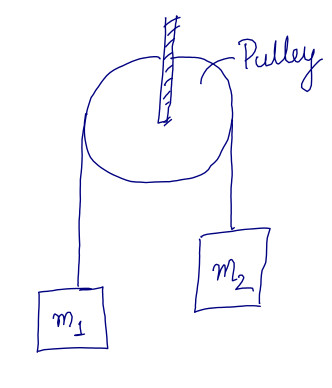
\includegraphics[scale=.5]{fbdpulley}
\centering
\end{figure}
\end{enumerate}
\end{document}
